% Created 2022-12-15 Thu 08:13
% Intended LaTeX compiler: pdflatex
\documentclass[11pt]{article}
\usepackage[utf8]{inputenc}
\usepackage[T1]{fontenc}
\usepackage{graphicx}
\usepackage{longtable}
\usepackage{wrapfig}
\usepackage{rotating}
\usepackage[normalem]{ulem}
\usepackage{amsmath}
\usepackage{amssymb}
\usepackage{capt-of}
\usepackage{hyperref}
\author{\textcopyleft}
\date{\today}
\title{Kolokwium1}
\hypersetup{
 pdfauthor={\textcopyleft},
 pdftitle={Kolokwium1},
 pdfkeywords={},
 pdfsubject={},
 pdfcreator={Emacs 28.2.50 (Org mode 9.6)}, 
 pdflang={English}}
\begin{document}

\maketitle
\tableofcontents

\begin{enumerate}
\item Nazwij dwa naturalne materiały półprzewdnikowe:\\\empty
Krzem, german
\item Co to jest elektron wlanecyjny?\\\empty
Elekton znajdujący się na ostatniej, najbardziej zewnętrznej warstwie atomu.
\item Rodzaje diod
Uniwerslane, prostownicze, impulsowe
\item Co to jest rekombinacja?\\\empty
Połączenie się pary cząstek lub jonów o prezeciwnych ładunkach elektrycznych, proces odwrotny do jonizacji.
\item harakterystka cześtotliwościowo ampitudową wzmacniacza tranzystorowego \begin{center}
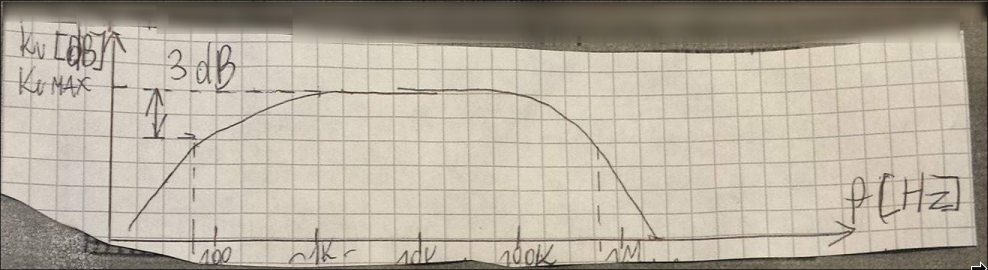
\includegraphics[width=.9\linewidth]{charakterystkaczestotliwosociowamipitudowa.png}
\end{center}
\item W jakim paśmie energetycznym występują elektrony swobodne?\\\empty
W paśmie przewodzenia
\item Rezystor w obwodzie emitera obniża wzmocninie napięciowe wzmcniacza w układzie? (Tak/Nie)
\item Narysuj energetyczne modele pasmowe półprzewdnika, izolatora i przewodnika \begin{center}
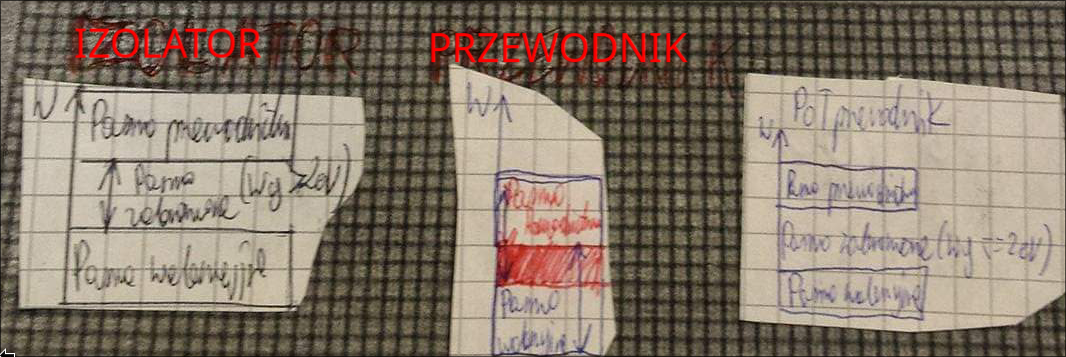
\includegraphics[width=.9\linewidth]{modelepasmowe.png}
\end{center}
\item Co to jest rezystancja dynamiczna (definicja i wzór)?\\\empty
Rezystancja jaką wnosi dioda w obwód prądu zmiennego, gdzie występuja niewielkie wzrosty składowej. \(R_d=\frac{U_2-U_1}{I_2-I_1}\)
\item Jak uzyskać półprzewdnik typu n?\\\empty
Poprzez domieszkowanie donorowe
\item Narysuj symbol diody zenera i oznacz końcowki\\\empty
\begin{center}
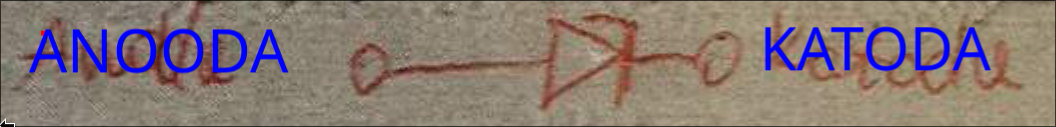
\includegraphics[width=.9\linewidth]{diodazenera.png}
\end{center}
\item Jakie nośniki są więkoszościowe w połprzewodniku typu p?\\\empty
Dziury
\item Bariera potencjału jest większa dla krzemu czy germanu?\\\empty
Krzemu.
\item Jaka jest przybliżna wartość wzmocnienia napięciowego wtórnika emiterowego?
\item Podaj określenie mocy admisyjnej\\\empty
Maksymalna moc strat. Maksymalna wartość iloczynu prądu i napięcia stałego, przy którym dioda może pracować.
\item Nazwij rodzaje przebica złącza p--n przy polaryzacji zaporowej.\\\empty
Zenera, elektryczne
\item Jakie daw podstawowe tory (obwody) wyróznia się we wzacniaczu trazystorowym?
\item Przy jakiej polaryzacji złącz bramka--kanał pracuje tranzystor polowy złączowy?\\\empty
Polaryzacja zaporowa.
\item Transport nośników w obszarze kanału tranzystora polowego musi sie odbywać w kierunku od \textbf{źródła} do \textbf{drenu}.
\item Wymień przynajmniej dwa układy polaryzxacji tranzystora bipolarnego.\\\empty
Stałym prądem baazy, emitera
\item Narysuj symbol tranzystora biploarnego i oznacz końcówki.\\\empty
\begin{left}
\centering
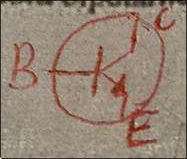
\includegraphics[width=50]{tranzystorBipolaarny.png}
\end{left}
\item Wymień prznajmniej dwa zakresy pracy tranzystora bipolarnego.\\\empty
0E, 0B, 0C
\item Aby tranzystor biploarny posiadał zdolności wzmacniające, złącze BE musi być spolaryzowane w kierunku \textbf{przewodzenia}, a złącze BC musi być spolaryzowane w kierunku \textbf{zaporowym}.
\item \(I_B = 8\mu A\) oraz \(I_C = 0.64mA\), Wyznacz \(B_N\)
\item Nazwij ikłady włączenia tranzystora bipolarnego.\\\empty
Ze wspólnym emiterem, kolektorem, bazą
\end{enumerate}
\end{document}